\begin{frame}[noframenumbering,plain]
    \setcounter{framenumber}{1}
    \maketitle
\end{frame}

\section{Содержание}

\begin{frame}{Содержание}
	\LARGE
	\begin{enumerate}
		\item Введение
		\item Математические модели
		\item Численный алгоритм решения
		\item Программный комплекс NonLocFEM
		\item Анализ решений
		\item Заключение
	\end{enumerate}
    %\tableofcontents
\end{frame}

\section{Введение}
\begin{frame}
	\centering
	\Huge
	Введение
\end{frame}

\begin{frame}{Введение}
	\begin{minipage}{0.39\textwidth}
	\begin{center}
		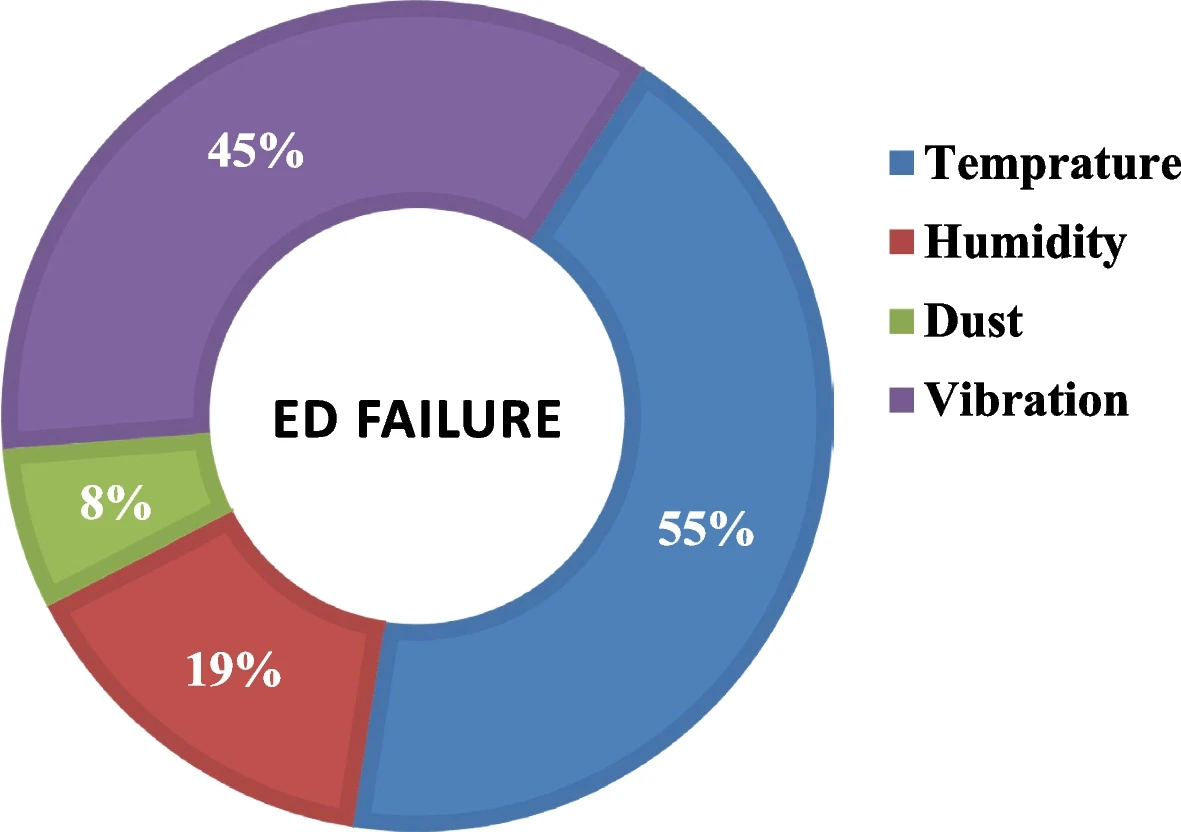
\includegraphics[width=\linewidth]{pics/EquipmentFailure.png} \\
		Причина выхода из строя микроэлектроники
	\end{center}
	\end{minipage}
	\hfill
	\begin{minipage}{0.59\textwidth}
		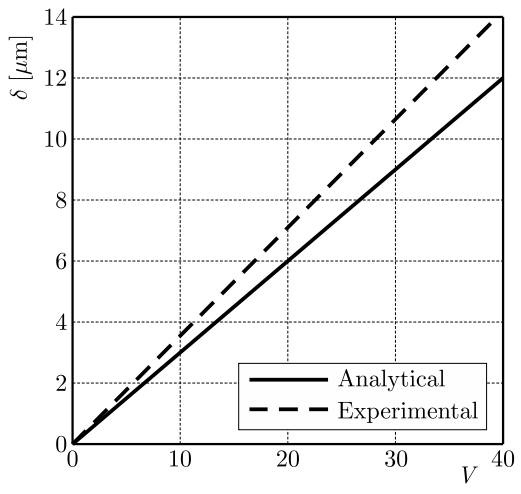
\includegraphics[width=0.49\linewidth]{pics/VoltageVariation.png}
		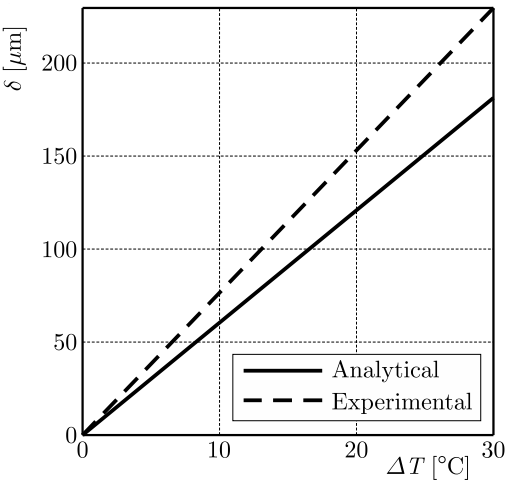
\includegraphics[width=0.49\linewidth]{pics/TemperatureVariation.png} \\
		Отклонение наконечника привода при увеличении вольтажа и температуры
	\end{minipage}
	
	\bigskip	
	
	Изображения взяты из источников:
	\begin{itemize}
		\justifying
		\item Amir R. Life Expectancy of Electronic Equipment Post-Loss.
		\item Pourrostami H., Viliani N. Study of a MEMS hybrid thermo-PZT micro actuator // Journal of Theoretical and Applied Mechanics. 2016. Vol. 54. P. 1309--1318. DOI: 10.15632/jtam-pl.54.4.1309. 
	\end{itemize}
\end{frame}

\begin{frame}
	\begin{minipage}{0.29\textwidth}
		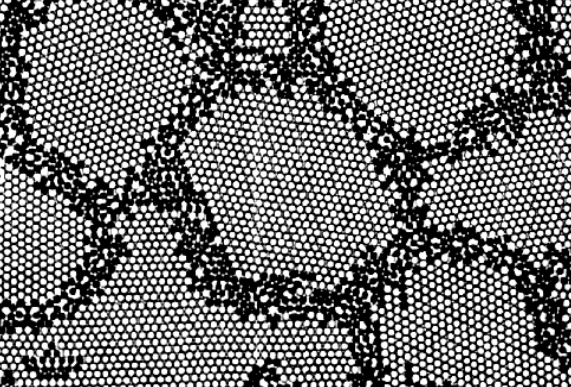
\includegraphics[width=\linewidth]{pics/Atoms.png} \\
		\medskip
		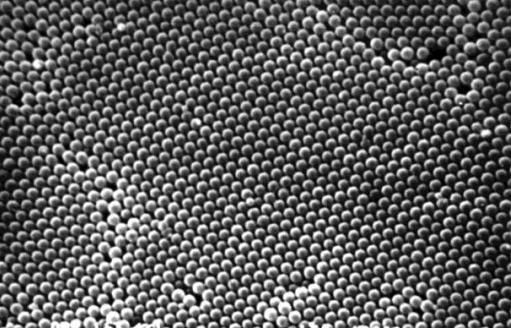
\includegraphics[width=\linewidth]{pics/Kremnezem.png} \\
		Атомные решётки материалов
	\end{minipage}
	\hfill
	\begin{minipage}{0.69\textwidth}
		\begin{center}
		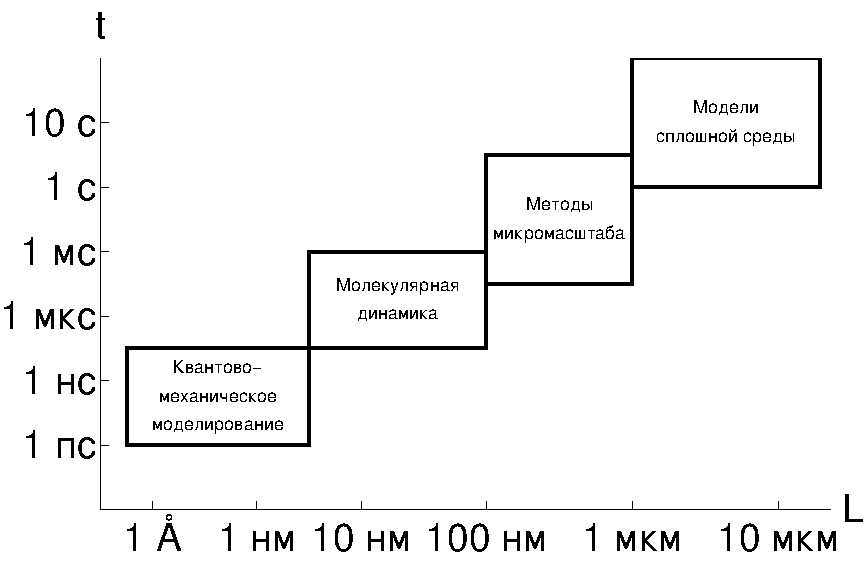
\includegraphics[width=\textwidth]{pics/ModelsHierarchy.pdf} \\
		Иерархия моделей моделей механики твёрдого тела
		\end{center}
	\end{minipage}
	
	\bigskip	
	
	Изображения взяты из источников:
\begin{itemize}
	\justifying
	\item Гусев А. И. Наноматериалы, наноструктуры, нанотехнологии. М.: ФИЗМАТЛИТ, 2005. 416 с. ІЅВN 5-9221-0582-5.
	\item Наноматериалы и нанотехнологии / В.М. Анищик [и др.] ; под ред. В.Е. Борисенко, Н.К. Толочко. Минск : Изд. центр БГУ, 2008. 375 с. ІЅВN 978-985-476-618-8.
\end{itemize}
\end{frame}

\begin{frame}{Модели обобщённой механики сплошной среды}
	Модели сплошной среды, учитывающие структуру материала:
	\begin{itemize}
		\item \textbf{моментные модели}:
		\begin{itemize}
			\justifying
			\item \textbf{микрополярные} (Eugène и François Cosserat, V.~G{\"u}nther, Э.Л.~Аэро, Е.В.~Кувшинский, Никабадзе~М.У. и др.);
			\item \textbf{микроморфные} (R.D.~Mindlin, A.C.~Eringen и др.);
		\end{itemize}
		\item \textbf{дальнодействующие эффекты}:
		\begin{itemize}
			\justifying
			\item \textbf{градиентные} (R.A.~Toupin, R.D.~Mindlin, E.C.~Aifantis, С.А.~Лурье, В.В.~Васильев и др.);
			\item \textbf{нелокальные} (E.~Kr{\"o}ner, A.C.~Eringen, D.~Rogula, D.G.B.~Edelen, S.B.~Altan, C.~Polizzoto, A.~Pisano, Г.Н.~Кувыркин, В.С.~Зарубин, И.Ю.~Савельева и др.);
		\end{itemize}
	\end{itemize}
	
	\justifying
	\bigskip
	\textbf{Цель работы} --- исследовать особенности \textbf{нелокальных} моделей теплопроводности и термоупругости, разработать собственный программный комплекс.
	
	\begin{minipage}{0.32\linewidth}\centering
		
\includegraphics[width=\textwidth]{pics/ansys.pdf}
	\end{minipage}
    \hfill
    \begin{minipage}{0.32\linewidth}\centering
        
\includegraphics[width=\linewidth]{pics/abaqus.pdf}
    \end{minipage}
    \hfill
    \begin{minipage}{0.32\linewidth}\centering
        
\includegraphics[width=\linewidth]{pics/FeNiCs.png}
    \end{minipage}
\end{frame}

\begin{frame}
    \frametitle{Положения, выносимые на защиту}
    \begin{itemize}
    	\justifying
        \item Модели нелокальной теплопроводности и термоупругости, позволяющие описать процессы передачи теплоты и напряжённо-деформированного состояния в материалах с микро- и наноструктурой.
        \item Новые численные алгоритмы решения на основе метода конечных элементов, адапатированные под многопроцессорные вычислительные системы.
        \item Собственный программный комплекс NonLocFEM, в рамках которого реализованы все рассматриваемые в работе методы решений.
    \end{itemize}
\end{frame}
\note{
    Проговариваются вслух положения, выносимые на защиту
}
